\section{Introduction to the Closure problem and theoretical solutions}
\label{sec:closure}


The averaged equations derived previously need what we call closure terms to be solvable. 
In this section, we outline them from the lowest order to the higher ones, i.e. from the most relevant to the smaller ones.
Note that the importance of higher order terms become more and more important, as the suspension get nonuniform. 
Likewise, we start by revealing the closures of the fluid-phase average (\ref{eq:favgsp}) and particulate-phase average for rigid particles (\ref{eq:pavgsp}). 
Then, we discuss the implication of the deformable and non-uniform particles distribution model. 
Lastly, the closure problem for the PBE (\ref{eq:PBM_QBMM}) will be discussed. 
\tb{Read morel book there is a lot of hints on the closures terms for Hybrid models and surface tension}

\tb{exprimer sigma en fonction des fluctuations and find something interesting}

\subsection{The averaged drag force term}
In this part we focus on the drag force term $n\left<\bm{f}_\alpha\right>^p$ appearing in both, particulate-phase and fluid-phase average.
It represents the drag force generated by the fluid phase on the dispersed phase and vice versa.
Therefore, it appears with a minus sign in the fluid average and a positive sign in the particulate average.  
This term is of most importance since it is  a zeroth order term. 
Unlike the other closure terms which are all first order or more. 
\tb{How to define properly the order ?}
Thus, accurate empirical formulas must be provided to predict its value for a set of dimensionless numbers, namely, $Ga$, $Bo$, $\mu_r$ and $\phi$ (that is the aim of \ref{chap:DNS} where we close this terms by use of DNS). 
This force is composed of a hydrodynamical part $\bm{f}^h$ and a contact force $\bm{f}^{b}$.
Consequently, $\left<\bm{f}\right>^p=\left<\bm{f}^h\right>^p+\left<\bm{f}^b\right>^p$.
Many author tried to close this term by deriving the theoretical expression of the drag force.
For solid spherical particles \cite{jackson1997locally} and \cite{zhang1994ensemble} found in the limit of Stokes and dilute flows a closure.
In dilute flow $\bm{f}^b_\alpha$ is negligible since there is no contact between particles.
In addition, in dilute flow the particles experience a drag forces due to the fluid as if they were isolated from the other particles. 
Besides, in Stokes flow the well known formula of the Stokes drag force on an isolated sphere is given by, $\bm{f}_\alpha^h =  6\pi\mu L/2(\bm{u}_\alpha - \bm{u})$, where $\bm{u}$ is the velocity of the fluid phase at the same position. 
Thanks to those assumptions, a closure is possible. 
Nevertheless, the hypothesis are very restrictive, therefore we need to investigate more accurate closure terms for droplets or bubbly dispersed phase. 
In the following we present semi-empirical model of the averaged drag force for isolated particles.
\citet{loth2008drag}, considered solid deformable particles which is a first step though deformable droplets. 
Later, we can find a lot of semi-empirical expression to express the drag coefficients on bubbles (see \citet[Appendix B]{gemello2018modelling}). 
Indeed, the most used correlation is the one of \citet{tomiyama1998drag}, where they derive an expression for the drag coefficient of a deformable bubble. 
It yields,
\begin{equation}
    C_D = \max\left\{
        \min\left[
        \frac{24}{Re}\left(
            1 + 0.15Re^{0.687}
        \right),
        \frac{48}{Re}  
        \right],
        \frac{8Bo}{3(4+Bo)}
    \right\}.
\end{equation}
This correlation is the merging of several correlation valid in given limits.
Therefore, this correlation is valid in every regime.
\citet{tomiyama1998drag}'s drag law has been used widely in the modeling of bubble columns to close the averaged equations of the Euler-Euler model \citep{sporleder2012population}. 
Even though a droplet is close to a bubble in a certain limit (i.e. when $\rho_r = 0$ and $\mu_r = 0$) it is still very inaccurate to use this correlation for droplets. 
In stokes flows \citet{dolata2021faxen} derived the drag force on a spherical and deformable droplet thanks to boundary integral methods (BIM) (see \citet{pozrikidis1992boundary} for more information on BIM).
In inertial regime no theoretical expression can be found in the literature.
However, in \citet{magnaudet1997forces} they perform a complete review of the current stat of the art regarding the drag force term form low to moderate Reynolds numbers. 

Up to now we have considered the drag force on an isolated particle.
Nevertheless, as mentioned below this assumption is only valid in the dilute cases.
The dilute limit is archived for $\phi \le 0.03$ for solid spherical particle in stokes regime (according to the validity of Einstein equivalent viscosity \citet{einstein1905neue}). 
We can suppose that it is the same scale for droplets. 
For greater $\phi$ the drag coefficient must be weighted by a term function of $\phi$.
At the origin \citet{di1994voidage} used the \textit{Voidage function} to accomplish this task.
It is presented as a function $g(\phi,Re)$ equivalent to the ratio between the non-isolated drag force over the isolated drag force.
However, it has been derived for solid spherical particles and not for droplets. 
A more used formalism for bubbly flows is what we call, the swarm factor, originally from \citet{richardson1997sedimentation}, it is the factor between the isolated drag coefficient and actual drag coefficient.
\citet{richardson1997sedimentation} conducted experiment on segmenting solid particles and deduce the following correlation for the swarm factor,
\begin{equation}
    \frac{C_d}{C_d^{\infty}} = (1-\phi)^n
\end{equation}
where, $C_d^{\infty}$ is the drag coefficient on an isolated particle and $n$ is a constant depending on the nature of the dispersed phase (see \citet[Appendix B]{gemello2018modelling} for a complete discussion).
In \citet{sporleder2012population} they use this swarm factor to carry out Euler-Euler simulation.
In \citet{roghair2011drag} they derive a swarm factor considering deformable particles, it yields,
\begin{equation}
    \frac{C_d}{C_d^{\infty}} = \left(1+\frac{18\phi}{Bo}\right)(1-\phi),
\end{equation}
where we can notice the dependency with the \textit{Bond number} characterizing the deformability. 
Other swarm factors are available in the literature.
However, most of them have been validated for air-water system. 
So they still need validation for other system such as emulsions.
To conclude, the drag force closure term has been widely investigated for bubbly flows but no study could be found for emulsion. 
Consequently, there is a clear need for accurate model of the averaged drag force, either isolated or in dense configuration. 
\cite{fox2012large}

\subsection{The stress term}
In the case of rigid dispersed phase and Newtonian fluid for the fluid phase we can define the stress tensor as $\left<\bm{\sigma}\right>^f = -(1-\phi)\left<p\right> + 2\mu\left<\bm{e}\right>$, where $p$ is the pressure and $\bm{e}$ the rate of strain tensor. 

\subsection{The particle-fluid-particle stress \tb{and particule-particule stress}}

In \citet{nott2011suspension} they demonstrate that in \ref{eq:pavgsp} the source terms $\left<\bm{f}_\alpha\right>^p$ can be decomposed into a pure drag force and a divergence of a stress, namely, $\left<\bm{f}_\alpha\right>^p  
= \left<\bm{f}^{\text{drag}}_\alpha\right>^p
+\bm{\nabla (n\left<\sigma\right>^p)}$. 
The latter term would be responsible for particle migration in suspension or emulsions \citep[Chapter 7]{guazzelli2011}.
Therefore, it is a key feature that cannot be omitted. 
In stokes flows \cite{nott2011suspension}, derived a formulation for this stress, called the \textit{particle stress}.
It has the following form. 
We note $\bm{y}^m_{\alpha \beta}$ the middle point between the particles $\beta$ and $\alpha$ of center of mass $\bm{y}_\beta$ and $\bm{y}_\alpha$. 
Then, the expression for the hydrodynamical contribution of the particle stress is,
\begin{equation}
    \label{eq:PFP}
    n\left<\bm{\sigma}^h\right>^p
    = \sum_\alpha g_\alpha \sum_\beta (\bm{y}^m_{\alpha \beta} - \bm{y}_\alpha)\bm{f}^h_{\alpha \beta}
    -1/2\bm{\nabla}\cdot \sum_\alpha g_\alpha \sum_\beta (\bm{y}_{\alpha \beta} - \bm{y}_\alpha) (\bm{y}_{\alpha \beta} - \bm{y}_\alpha)\bm{f}^h_{\alpha \beta} 
    + \ldots
\end{equation}
where, $\bm{f}^h_{\alpha \beta}$ is the hydrodynamical force applied on the particle $\alpha$, due to the motion of the particle $\beta$ (since stokes flows are linear we can decompose each contribution of any particles). 
Besides, it can be show that the total particle stress reads as, $\left<\bm{\sigma}\right>^p = \left<\bm{\sigma}^h\right>^p+\left<\bm{\sigma}^b\right>^p$, where the superscript $^b$ stand for the contact force between particles and $^h$ for hydrodynamical contribution.
Indeed, not only hydrodynamical stress play a role in the particles stress, but also the contact forces between particles generate a stress (the authors also considered long range inter particular forces which gives rise to another stress tensor of similar nature).  
It is important to note that only the hydrodynamical forces contribute to the pure drag forces. 
As a matter of fact the inter particular forces cancel with each other according to Newton second law of motion, therefore the pure drag component is null.
This study make use of volume average method to derive the PFP stress. 
While, in \citet{zhang2021ensemble} they derive an expression of the PFP with ensemble average method without the assumption of stokes flow.
It turns out that their expression correspond to the first order of the previous one. 
Indeed, the summation on $j$ in equations \ref{eq:PFP} reduce to the summation over the nearest particle, thus it reads as,
\begin{equation}
    \Sigma_{PFP} = \frac{1}{2}  \sum_\alpha (\bm{y}_\beta - \bm{y}_\alpha)\bm{f}_\alpha,
\end{equation}
here, $\beta$ is the label of the nearest particle from the particle $\alpha$. 
Up to now this closure term has always been neglected in Euler-Euler simulations. 
However, recent investigation by \citet{wang2021numerical} confirm that this term can indeed predict the migration and the drifting kissing tumbling mechanism of the dispersed phase.
Consequently, it is of great interest to study this new feature in droplets suspension. 

\subsection{The fluctuations terms}
\tb{derive here the transport of the fluctuation see \citet{nott}}
In \ref{eq:favgsp}, \ref{eq:pavgsp} and \ref{eq:Iavg} we can notice average of the product of fluctuations appearing on the right hands side, respectively,
\begin{equation}
    \left<\bm{u'u'}\right>^f, \;\;\;\left<\bm{u'}_\alpha \bm{u'}_\alpha\right>^p, \;\;\;\left<\bm{u'}_\alpha \bm{\omega}'_\alpha\right>^p,
\end{equation} 
Indeed, all the product of microscale variables $\left<\bm{uu}\right>$ can be rewritten as a product of average plus the average of fluctuations, namely, $\left<\bm{uu}\right> = \left<\bm{u}\right>\left<\bm{u}\right> + \left<\bm{u'u'}\right>$ for the velocity. 
We recall that we solve the averaged equation for the averaged variables, thus the product of the fluctuations is unknown.
And since the velocity fluctuations plays a key role in the averaged equations it is of interest to study turbulence in more details. 
The fluctuation tensor presented above is not to be confused with the actual turbulent Reynolds stress arising at high Reynolds number. 
Indeed, there is different scale of turbulence well distinguishable. 
In \cite[Figure 1]{balachandar2009scaling} they show the energy spectra of a suspension at different scale.
We can clearly identify the pseudo-turbulence at the scale of the particles and the more \textit{classical} turbulences phenomenons arising at smaller scale. 
By classic turbulence we mean the turbulence which exist even in the absence of dispersed phase. 
This turbulence exists from Kolmogorov to integral scale eddies. 
Where the pseudo turbulence arise at the scale of the particle.
Nevertheless, even though it is not the same scale the phenomenon is exactly the same, i.e. fluctuation of the velocity around a mean resolved velocity. 
In \citet{mehrabadi2015pseudo} they demonstrate that for gas-fluid system the pseudo-turbulence arising from the presence of particles is irrespective from the classic turbulence. 
Also, in \citet{risso2018agitation} they quantify the effect of both kind of turbulence for bubbly flow and conclude that the two phenomenons where weakly correlated. 
Which means that the scaling of the pseudo turbulence is conserved even in the presence of smaller scale turbulence. 
Consequently, in this thesis we won't consider small scale turbulence but only particles scale turbulence. 
Since the derivation of a theoretical model is not possible in the case of pseudo turbulence we investigate this terms with the use of DNS in the next chapter.
Even though turbulence and pseudo turbulence are not the same thing, a lot of authors use the classic turbulence models to account for pseudo turbulence phenomenons. 
Indeed, in \citet{gemello2018modelling} they explain how to make the link between the two conceptual framework.
Regardless of the models, often the authors use a transport equation for the pseudo turbulence tensor \citep{du2022analysis} just like with the $k-\omega$ models and other turbulent models. 
\subsection{Consideration of poly sized distribution and deformability.}

Moreover, the consideration of the poly dispersion of the emulsion and deformability of the droplets bring in to place two additional kind of unclosed terms.
Indeed, we first see appear this terms linked to the drops size fluctuation.
If we consider only the mass and momentum conservation equations, we found,
\begin{equation}
    \left<V_\alpha' \bm{u}_\alpha'\bm{u}_\alpha'\right>^p,\;\;\;
    \left<V_\alpha' \bm{u}_\alpha'\right>^p.
\end{equation} 
From out knowledge no study have been studying those fluctuation terms.
Indeed, all attempts to model poly dispersed suspension or emulsion neglected it. 
However, there are first order terms, as the preceding fluctuation terms, which were not negligible.
That is why it is highly probable that those terms are significant.
These terms solely arises from the poly sized nature of the suspension.
The deformation of the droplets, i.e. the internal fluctuation of the velocity fields, bring two additional closure.
Namely,
\begin{equation}
    \left<\int_{V_\alpha} \bm{w}_\alpha dV\right>^p,\;\;\;
    \left<\bm{u_\alpha}'\left(\int_{V_\alpha} \bm{w}_\alpha dV\right)'\right>^p,
\end{equation}
which represent respectively, the averaged internal fluctuation of the drops and the fluctuation of the internal fluctuation of the drops.
Note that the former term appear as a factor of the mean velocity $\left<\bm{u}_\alpha\right>^P$ in the momentum balance equations. 
Which is quite different from the other closure terms which are all source terms.
Therefore, it might have a great influence into the equations. 
As seen previously the fluctuations of the droplet can be decomposed into an expansion around the center of the particles.  
Considering, only first two terms in the expansion it reads (see \ref{ap:cinematic}), 
\begin{equation}
    \int_{V_\alpha} \bm{w}_\alpha dV
    =  \bm{\nabla u}|_{y_\alpha} \int_{V_\alpha} \bm{r}_\alpha dV
    +  \frac{1}{2}\bm{\nabla\nabla u}|_{y_\alpha} \int_{V_\alpha} \bm{r}_\alpha\bm{r}_\alpha dV
    + \ldots
\end{equation}
Note that the first term cancel out thus only second order fluctuations are non-negligible. 
Then, is it useful to consider higher order than the first one in the velocity expansion ? 
Knowing that the other closures are kept of order one maximum it might be coherent to neglect those.
To answer this question, computation of those closures will be carried out in the next chapter. 

\subsection{First and higher moments}
In the fluid-phase average, the last contribution to the bulk stress from the particles are the hydrodynamic moments.
In practice, even the first moment is rarely implemented in Euler-Euler models, since it is not trivial to compute, and almost no model exist.
Therefore, we will only focus on the first moment and neglect the higher ones (which is a reasonable assumption considering the good separation of scale). 
As mentioned earlier the first moment tensor is the sum of a symmetric tensor called the stresslet, and of an antisymmetric one which is related to the torque.  
The former has its importance in certain cases.
Indeed, when shear flow is dominant this tensor become non-negligible.
For example, one can derive the expression of the bulk viscosity of a dilute suspension of solid spheres, by using the expression of the stresslet tensor \citep{einstein1905neue}. 
In the case of mono disperse ascending droplets, it might be however negligible as there is no global strain since all the droplets are rising at the same speed (since they experience the same buoyancy).
However, for poly disperse emulsion we can expect strain generated by the different rising velocity of the droplets. 
Similarly, the antisymmetric part of the first moment, or the averaged torque, should be in average null for mono disperse suspension, while it might not be for poly disperse ones.
Theoretically, it is possible t derive an expression for the first moment on rigid spherical particles in stokes flows, see \cite{guazzelli2011}. 
Moreover, in \citet{dolata2021faxen}, thanks to Boundary Integral Method (BIM), they derive an expression for the first moment considering deformable particles through Faxèn laws.
Nevertheless, it is still very restrictive, and a theoretical closure or semi-empirical closure in a more general case might never be possible. 
Consequently, this closure term will be investigated in \ref{chap:DNS} and empirical closure will be proposed.  

\subsection{The source term J in the Population balance equations.}
As said in the first part, $J(\mathcal{\bm{R}},t)d\mathcal{R}$, is the rate of generation of entities. 
It encapsulates two phenomenons, the net rate of birth of entities, $B(\mathcal{\bm{R}},t)d\mathcal{R}$, and the net rate of death of entities, $D(\mathcal{\bm{R}},t)d\mathcal{R}$.
$B$ and $D$ represent respectively the break-up and the coalescence source term of the droplets. 
As said previously the hard part in solving the PBE is to find an accurate expression of these terms. 
It is indeed a very tough task since no accurate closure are available for droplets. 
Therefore, we limit ourselves to the study of coalescence phenomenons only, and discard the modeling of break up. 
In the following, we review the current state of the literature providing coalescence kernels models.  
The source term $B(\mathcal{\bm{R}},t)d\mathcal{R}$ measure how the distribution $f$ is modified by coalescence events.
Similarly, the source term $\left<B\right>^\lambda_\gamma$ measure how the moments $\theta_\gamma$ are modified by the coalescence. 
For example, if we consider a drop of size $L_1$ and another of size $L_2$, the drop resulting of this coalescence event will have a diameter $(L_1^3 + L_2^3)^{1/3}$. 
Then, the decrease of $\theta_\gamma$ can be written as, 
\begin{equation}
    \Delta \theta_\gamma 
    = (L_1^3 + L_2^3)^{\gamma/3} -L_1^\gamma - L_2^\gamma
\end{equation}
Besides, the rate of coalescence can be expressed as the product between the rate of collision times a probability of coalescence. 
The former will be noted $C(L_1,L_2)$ and the latter $P(L_1,L_2)$. 
Then, we can express the weighted source term as \citep{KAMP20011363}, 
\begin{equation}
    \left<B\right>^\lambda_\gamma = \frac{1}{2}\int_{L_1}\int_{L_2} C(L_1,L_2)P(L_\alpha,L_2) \Delta \theta_\gamma dL_1 dL_2.
    \label{eq:cockerel}
\end{equation}
Therefore, the closure problem reduce to the finding of the frequency of collision per unit of volume and a probability of coalesce. 
The probability of coalesce term represent the probability that the film drainage process occurs during a collision, resulting in the coalescence of droplets. 
In the following parts we give some details on present models, of collision frequency and coalescence probability.

\subsubsection{Probability of coalescence and Film drainage}

The probability of coalescence is mainly driven by the famous, film drainage problem. 
The film drainage occur when two drops come close together.
At some point the surfaces of the droplets form a nearly flat film. 
Then the fluids between the two surfaces try to escape as the drops come closer. 
At this scale, lubrication forces are driving the process (\citet[Section 4.3]{guazzelli2011}). 
If those forces do not repeal the drops, then the surface get eventually closer.
Considering this scale, the molecular interaction are now involved, such as the Van Deer Walls forces.
To model this phenomenon we often use the disjointing pressure into the film drainage equations (see \citet{de2015gouttes}). 
This is the global scheme of the situation. 
Now, we can dive into details to determine the actual probability of coalescence. 
In \citet[Figure 1]{chesters1991modelling} they summarize the conceptual framework of the coalescence source term. 
They show that the probability of coalescence problem can be divided into two sub-problems that are simpler. 
The first one is the modeling of the contact forces and motion of the particles during the approach in a given configuration.
The second is the modeling of the critical thickness of the film coalesce, i.e. the thickness above which the two drops merge.
The former will provide the actual time of interaction $t_i$. 
Together with the critical thickness, we can determine the critical time, $t_c$, it is then possible to define the probability of coalesce. 

The motion during the approach can be modeled by the lubrication forces theory.
The equations can be derived theoretically thanks to the hydrodynamical lubrication considering stokes flows.
Besides, there are different ways of approach for a pair of droplets, each way represent a different model \citep[Section 4.3]{guazzelli2011}. 
When two drops face each other, meaning that their respective velocities are pointing to the other particle's center of mass, it is called the squeezing problem.
When their velocities are opposite, but they do not point toward each other, this is called the shearing problem. 
The former situation present a singularity when the particles touch each other, while the second configuration doesn't. 
Also, another important parameter to consider, is to know if the particles are approaching each other at constant speed or constant acceleration.
In all cases it gives rise to different modeling frameworks.
That is why, is it of the most importance to study the actual collision behavior in the considered emulsions, in our case buoyancy driven flows.
For a better understanding of the methodology, we show below the development for the squeezing problem at constant velocity. 
\ref{fig:2drops} shows the problem at hand. 
The conservation of momentum equation for the fluid inside the film, it reads as,
\begin{equation*}
    - \frac{\partial p}{\partial r} 
    + \frac{\partial u_r}{\partial z^2} 
    = 0 
    \;\;\rightarrow 
    \;\; p \sim \mu_f u_r / h^2.
\end{equation*}
\begin{figure}[h!]
    \centering
    \begin{tikzpicture}
        \node (img) at (0,0){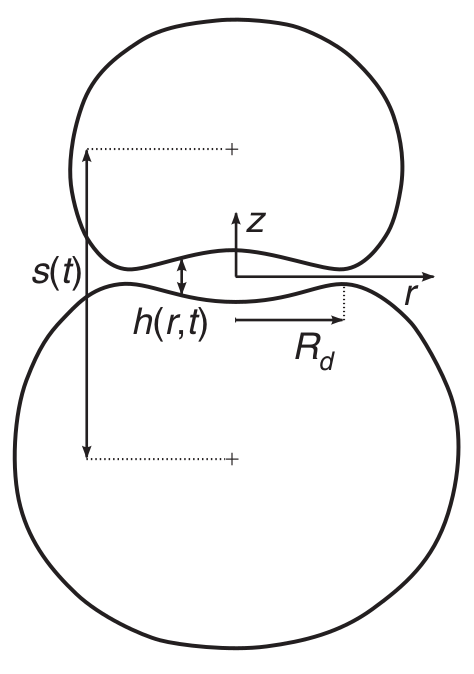
\includegraphics[width=0.2\textwidth]{image/pic/two-drops.png}};
        \draw[->](0.2,-1.2)--(0.2,-0.4)node[midway, right]{$U_{rel}$};
        \draw[<->](-0.12\textwidth,+0.02\textwidth)--++(0,-0.15\textwidth)node[midway, left]{$L$};
    \end{tikzpicture}
    \caption{Scheme of the squeezing problem with a dimple. Reprinted from \citet{kamp2017drop}.}
    \label{fig:2drops}
\end{figure}
Considering the mass conservation, i.e. $U_{rel} = -\frac{dh}{dt}$, where $U_{rel}$ is the relative velocity between the droplets. 
Then, applying the following scaling for the gradient term, $\frac{dh}{dt}\sim -h^3\gamma^2/(FL^2\mu_f)$, where $F$, is the force pushing the drops together, we get an expression for the thickness of the film $h$.
Namely, 
\begin{equation*}
    h \sim \left(\frac{\gamma^2t}{FL^2\mu_f}\right)^{-1/2}.
\end{equation*}
We obtain an equation which describe the evolution of the thickness of the film for a given configuration. 
Nevertheless, the force of approach stay unknown.
From this equation we can also determine the critical time at which the film breaks.
If define $h_c$ being the critical thickness, it follows,
\begin{equation}
    t_c \sim \frac{FL^2\mu_f}{\gamma^2h_c^2}.
\end{equation} 
However, note that the critical thickness is not known yet.
Note that here we considered the same diameter $L$ for each droplet. 
Others models have been developed taking other assumptions. 
We can cite again \citet{chesters1991modelling} which describe all the different regime, from deformable/mobile to rigid surfaces. 
Moreover, \cite{davis1989lubrication} present the theoretical framework to model the resistance force of two squeezing spherical particles.
They make use of both, boundary Integral Method  (BIM) \citep{pozrikidis1992boundary} and the lubrication theory.   
They suppose three different situations. 
The first one, where the particles are at moderate separation and/or high viscosity, and therefore, stay rigid. 
Then, they consider a deformable interface when the drops are relatively close and the viscosity ratio low. 
After, they study the limits where the interface is fully mobile.  
In each situation they conclude respectively that the force of resistance $F$ was :
$F\sim 1/L$ and  $F \sim \sqrt{d}$. 
The overall hypothesis is that $(a/h) Ca\ll 1$.
From the work of \citet{chesters1991modelling}, \citet{KAMP20011363} have derived models for poly-sized pairs of bubbles a derived a model function on the size ratio of the drops.
In \cite{leal2004flow} they observe experimentally the film drainage of two drops. 
They could conclude that the film will tends to have a dimple(i.e. the film is thicker in around the axis of revolution)  since the pressure is maximum at the center. 
Also, \citet{yiantsios1990buoyancy} studied poly disperse emulsion, they found that  the common phenomenon is that one small drops merge with a bigger one due to different buoyancy and therefore different velocity. 
Therefore, they analyzed with film drainage theory and boundary Integral method, the profile of deformation of the drop surface when getting close to a rigid interface (to represent the approach of a small drops toward a bigger one).
They conclude that a dimple is always formed and that the thinning rate scale as $h\sim 1/t^\alpha$.
$\alpha$ is a constant depending on where we evaluate $h$, indeed since there is a dimple there is a maximum thickness at the center of the film and a minimum one on the sides, the value of $\alpha$ are respectively $1/3$ and $2/3$ at the center and on the sides.
Many authors have worked on the topic since the last decay.
Here we only gave a glimpse of the lubrication theories. 
Nevertheless, to have a global overview of the film drainage problem we refer to \citet[Chapter 6]{leal2007advanced}.  

Next, we are interested in modeling the critical thickness, $h_c$.
To do so, one has to consider more complicated phenomenons.
Indeed, since $h_c$ arise at the microscopic scale, the model must include the disjointing pressure to the equilibrium equations. 
The classic expression for a planar film reads as, 
\begin{equation}
    \Pi(h) = \frac{A}{6\pi h^3},
\end{equation}
where $A$ is the Hamaker constant, its value depends on the material, but it scales around $10^{-10}J$ \citep{leal2007advanced}. 
Considering this new pressure balance, we can determine the minimum thickness $h_c$ below which the disjointing pressure is higher than the hydrodynamical pressure. 
The disjointing pressure attracts the surfaces of the film, consequently, it collapses and the droplets merge. 
It can be shown that $h_c$ scale as, 
\begin{equation}
    h_c \sim \left(\frac{L A}{24\pi\gamma}\right)^{1/3}Ca^{1/6}
\end{equation}
with $Ca$ the capillary number defined in introduction. 
This equation has been derived by \citet{chesters1991modelling} which first considered two droplets approaching with no deformation on the droplets surface.
Similarly, \citet{jones1978film} derived an expression for the minimum thickness for a droplet approaching a deformable interface instead of another drop. 
Besides, it is possible to consider deformation, more precisely to consider a dimple inside the film.
\citet{chesters1991modelling} and \citet{yoon2007coalescence} found similar formula for the critical thickness with the dimple model. 
If we consider fluctuations in the film then we refer to \citet{vrij1966possible}.
More complex model for viscoelastic film have been considered by \citet{bousfield1989thinning}.
Most of the authors mentioned above haven't considered inertial effect in the modeling of the film drainage problem. 
In \citet{sambath2019inertial} they investigated inertial drop collision with numerical simulation.
They consider Van-deer Val's forces in addition to inertial, capillarity and viscous forces.
Thanks to a Lagrangian-Eulerian method they can model length scale five order of magnitude below the radii length scale and resolve the film drainage properly including Vandar wals forces. 
They conclude that inertial delay the time of coalescence due to the bouncing between the two drops even tough the viscosity and density ratio is moderate. 
Therefore, plainly models need to be revisited while considering inertial effects.
Again, we will not make the list of all existing scaling theories since numerous articles have been published on this topic. 

Regardless of the hypothesis, the previous author provided on one hands models for the thickness of the film as a function of the time $h(t)$.
And on the other hands the critical value, $h_c$.
Therefore, it is possible to obtain a critical time of contact, $t_c$. 
Comparing the interaction time $t_i$ to the critical contact time gives the probability of coalescence.
The probability of coalescence for mono-sized pair of drops, reads, $P = \exp(-\frac{t_d}{t_i})$ \citep{chesters1991modelling}.
For poly sized-pair \citet{KAMP20011363} considered  $P = 0\;\;\text{if}\;\;t_d > t_i$ and $P = 1\;\;\text{if}\;\;t_d < t_i$.






\subsubsection{Collision frequency}

The other terms involved in the model of the coalescence source term, \ref{eq:cockerel}, is the collision frequency. 
\citet{chesters1991modelling} provide us with a general formulation of the collision frequency per unit of volume.
They assume mono-sized suspension of spherical particles. 
It reads, 
\begin{equation}
    C =  k v d^2 n^2,
\end{equation}
where $v$ is a characteristic velocity between two point located at a distance $d$ apart.
The value of $k$ and $v$ depends on the structure of the flow.
Indeed, for simple shear flow \citet{smoluchowski1917mathematical} show that, $v = \dot{\gamma} d$ and $k=2/3$, with $\dot{\gamma}$ the mean rate of strain. 
For turbulent flow \citet{saffman1956collision} give, $v = (\varepsilon/v)^{1/2} d$ and $k  = (2\pi/15)^{1/2}$.
In the context of gravity flows, \citet{davis1984rate} studied the rate of collision for gravity induced collisions.
They considered spherical particles of different size. 
When two particles come close Van der Waals forces tends to attract the drops together, thus doublets of particles is formed.
The rate at which doublets are formed is then calculated in the limit of high Péclet numbers (negligible Brownian motion) and small $Re$.
This rate is closely linked to the rate of collision in the limit where inertial effect are negligible. 
For a more general case,  \citet{zhang1991rate} considered Brownian collision and gravity induced collisions for poly-sized drops emulsion.
By solving the diffusion equation for relative Brownian motion of two drops, and following the relative motion of pairs of drops, they could determine theoretical expression of the collision efficiency.
The gravity induced collision rate neglecting inter particle forces is, 
\begin{equation}
    C = n_1n_2 v_{1} d_1^2 \pi   E_{12}(1-\lambda^2)(1+\lambda^2), 
\end{equation}
where, $n_1$ and $n_2$ is the number density for, respectively, drops of size $d_1$ and $d_2$.
$\lambda$ is size ratio of the drops.
$E_{12}$ is the collision efficiency. 
Note that $E_{12}$ tends to 0 as $\lambda$ goes to $0$ since the relative velocity of the drops tends to $0$ in this limit.
In \citet{zinchenko1994gravity} they solve numerically the Fokker-Planck equation for the pair distribution function. 
Then they give the expression of the collision efficiency for a wide range of Péclet number, viscosity and size ratio.
The Brownian  motion is shown to be negligible for $Pe< \mathcal{O}(10^2)$.
The influence of the van deer walls interaction is small except in the range of high drop-to-medium viscosity ratio.  
Even though numerical simulation of the diffusion equation provided closure for the collision frequency, it is essential to use DNS in order to provide empirical laws covering a wider range of parameters. 

Others closure for the coalescence kernels are available in \citet[Chapter 10]{morel2015mathematical}.
They make an overview of the current state of the modeling of the source term, $\left<B\right>$ for turbulent induced flows. 
However, even trough several models exist for turbulent bubbly flows, nothing is done for gravity induced flows of droplets. 
Therefore, the probability of coalescence and the collision frequency, need also to be determined trough DNS.
And empirical expression of the coalescence kernel need to be provided. 
In the next chapter we focus on the calculation of the closure terms trough DNS simulation preformed with the code Basilisk.